\documentclass[12pt]{article}
\usepackage[utf8]{inputenc}
\usepackage{graphicx}
\usepackage{mathtools}
\usepackage{amsmath}
\usepackage{amsfonts}
\usepackage{amssymb}
\usepackage{amsthm}
\usepackage{enumitem}
\usepackage{centernot}
\usepackage{marvosym}
\usepackage{lscape}
\let\marvosymLightning\Lightning
\newtheorem{theorem}{Theorem}
\newtheorem{corollary}{Corollary}[theorem]
\newtheorem*{remark}{Remark}
\newtheorem{innercustomthm}{Theorem}
\newenvironment{customthm}[1]
  {\renewcommand\theinnercustomthm{#1}\innercustomthm}
  {\endinnercustomthm}
\newcommand{\subscript}[2]{$#1 _ #2$}
\newcommand{\N}{\mathbb{N}}
\newcommand{\Z}{\mathbb{Z}}
\newcommand{\R}{\mathbb{R}}
\newcommand{\C}{\mathbb{C}}
\renewcommand\qedsymbol{QED}
\newcommand{\divby}{%
  \mathrel{\text{\vbox{\baselineskip.65ex\lineskiplimit0pt\hbox{.}\hbox{.}\hbox{.}}}}%
  }
\newcommand{\notdivby}{\centernot\divby}
\newcommand\setItemnumber[1]{\setcounter{enumi}{\numexpr#1-1\relax}}
\title{\scalebox{2}{Math 431 Homework 6}}
\author{\scalebox{1.5}{Theo Koss}}
\date{November 2020}
\begin{document}
\maketitle
\section{Problem 1}
Draw the lattice diagram for the power set of $X=\{a,b,c,d\}$.
\newline\scalebox{.13}{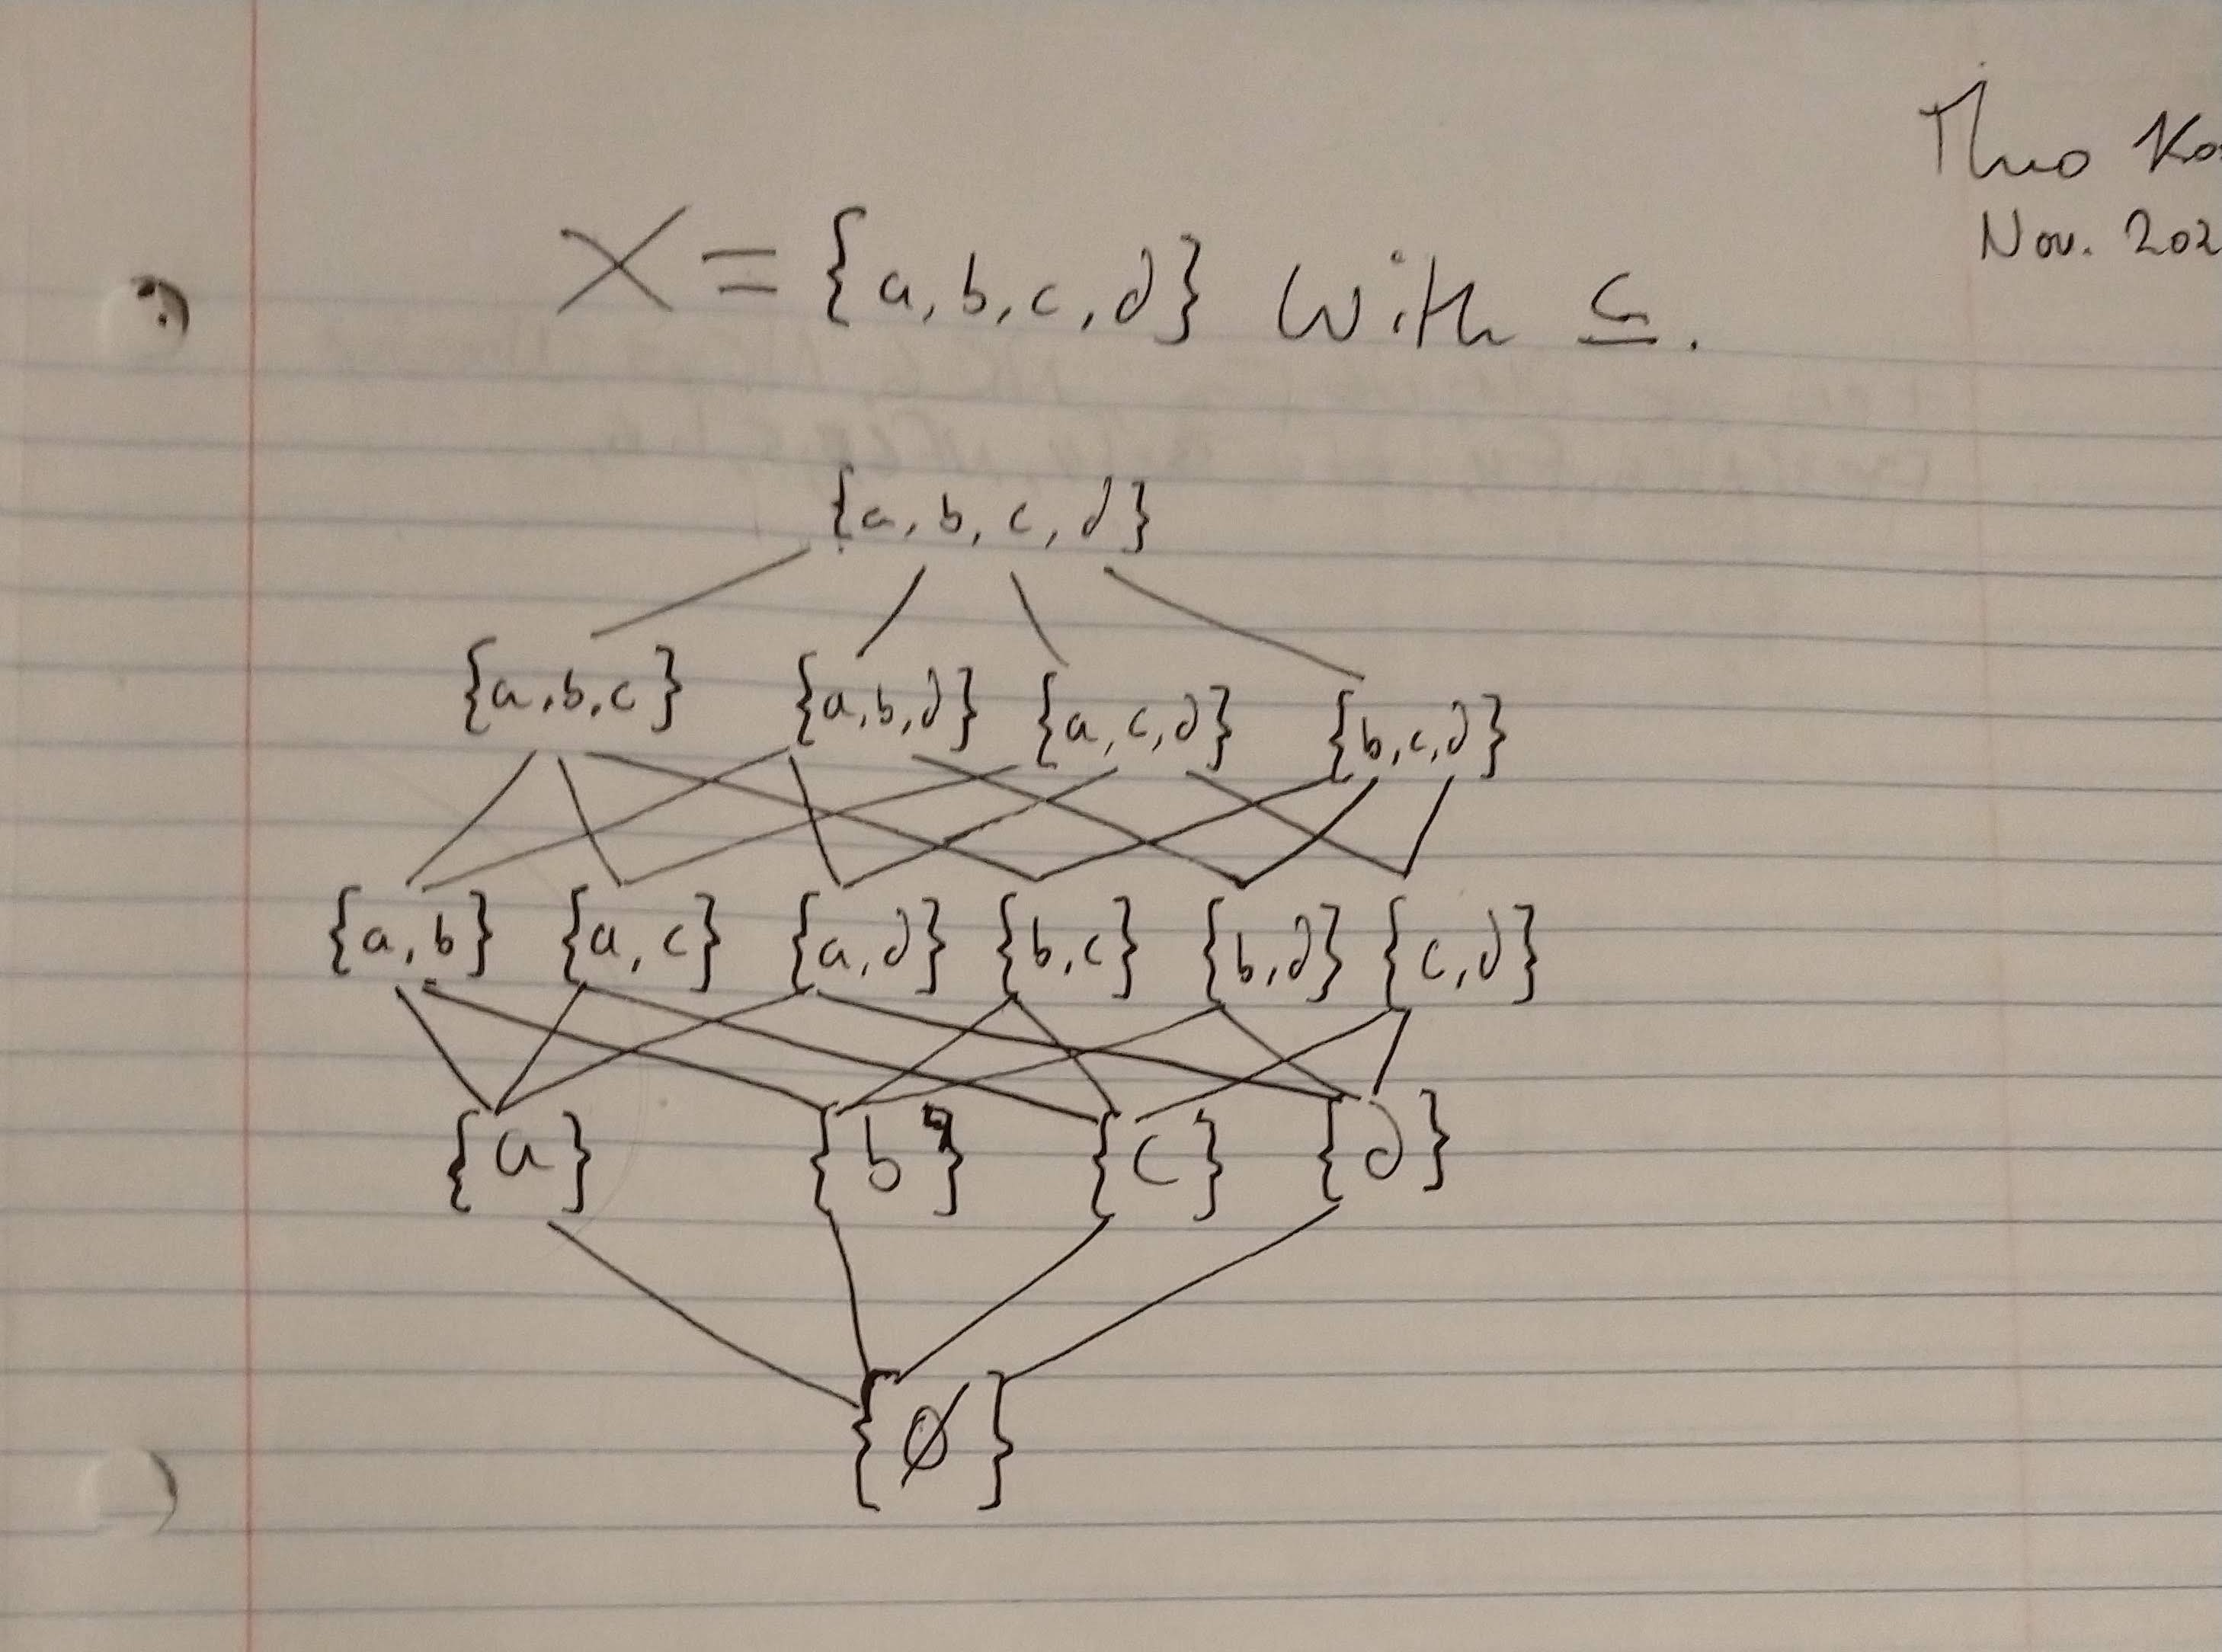
\includegraphics{Lattice}}
\section{Problem 2}
Let $B$ be the set of all positive integers that are divisors of 210. Define an order on $B$ by $a\preceq b$ iff $b\divby a$. Prove that $B$ is a Boolean Algebra. Find a set $X$ such that $B$ is isomorphic to $(P(X),\subseteq)$.
\begin{proof}First we will list out the elements of $B$, aka the divisors of 210. \newline $B=\{1,2,3,5,6,7,10,14,15,21,30,35,42,70,105,210\}$.\newline By definition 6.9, a lattice $B$ is a Boolean Algebra iff $B$ has a greatest element $I$ and smallest element $O$, such that $B$ is distributive and complemented.
    \newline \scalebox{.13}{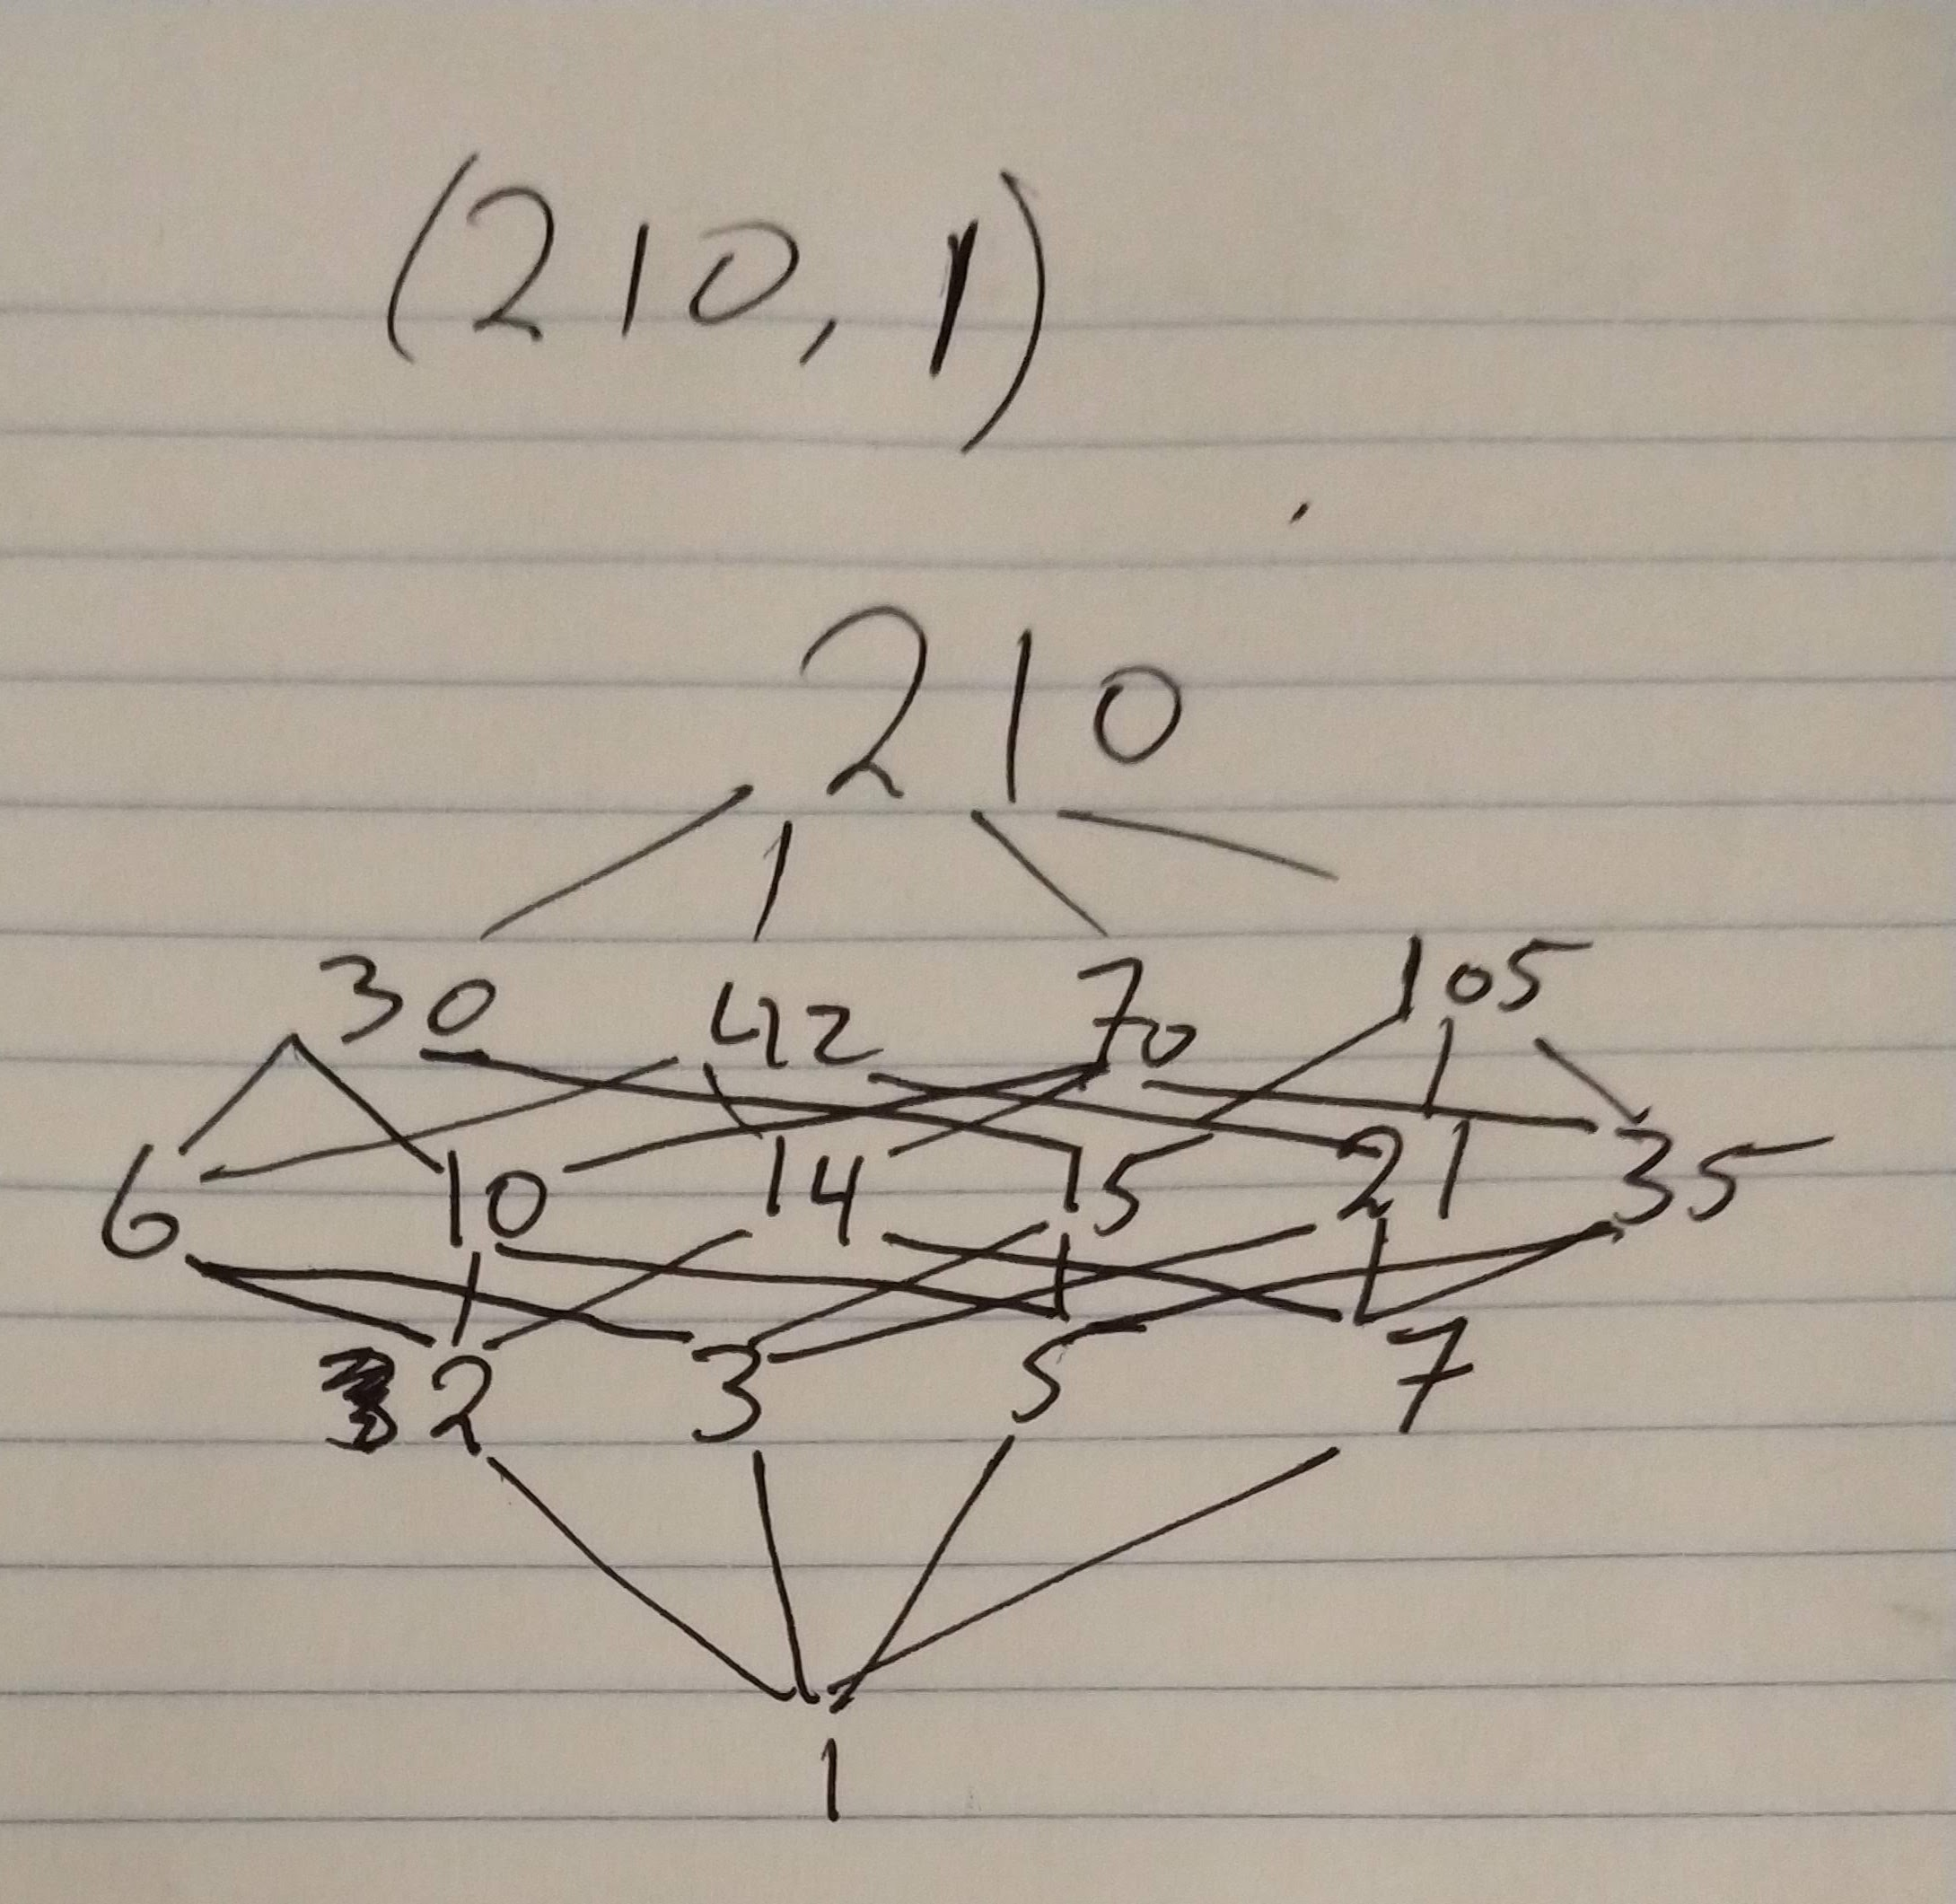
\includegraphics{210Lattice}}\begin{enumerate}
    \item Greatest and smallest element: Clearly, from the picture, $I=210$, $O=1$.
    \item Distributivity: \newline N2S: $\forall a,b,c\in B, a\wedge(b\vee c)=(a\wedge b)\vee(a\wedge c)$. $$a\wedge(b\vee c)=[a\wedge(a\vee c)]\wedge(b\vee c)$$ $$=a\wedge[(c\vee a)\wedge(b\vee c)]$$ $$=a\wedge[c\vee (a\wedge b)]$$ $$=a\wedge[(a\wedge b)\vee c]$$ $$=[(a\wedge b)\vee a]\vee[(a\wedge b)\vee c]$$ $$=(a\wedge b)\vee(a\wedge c)$$ As required.
    \item Complementivity (probably not a word but mathematicians make up words all the time): \newline N2S: $\forall a\in B, \exists a'\in B$ such that $a\vee a'=I$ and $a\wedge a'=O$. $\forall a\in B$, $a'=$\scalebox{1.3}{$\frac{210}{a}$}$\in B$. $a'$ is of course, an elements of $B$ because all divisors of 210 are in $B$.
\end{enumerate}
Therefore $B$ is a Boolean Algebra.
\end{proof}
The power set $P(X)$ with order $\subseteq$, and set $X=\{a,b,c,d\}$ is isomorphic to $B$. See problem 1 for the lattice, it is of the same structure, and is the same size, therefore it is isomorphic.
\section{Problem 3}
Draw the switching circuits for each of the following Boolean expressions:
\begin{enumerate}
    \item $(a\vee b\vee a')\wedge a$:\newline\scalebox{.5}{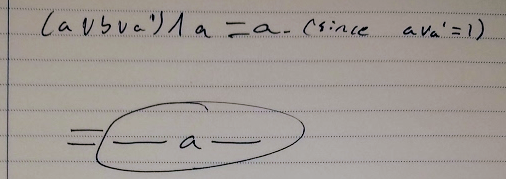
\includegraphics{Boolean1}}
    \item $(a\vee b)'\wedge(a\vee b)$:\newline\scalebox{.5}{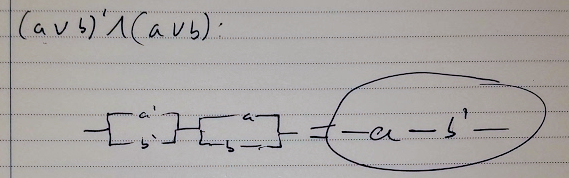
\includegraphics{Boolean2}}
    \item $a\vee(a\wedge b)$:\newline\scalebox{.5}{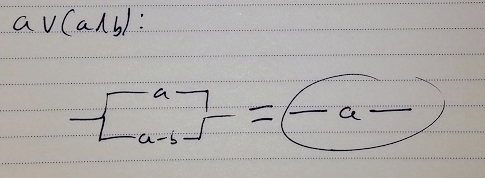
\includegraphics{Boolean3}}
    \item $(c\vee a\vee b)\wedge c'\wedge(a\vee b)'$:\newline\scalebox{.5}{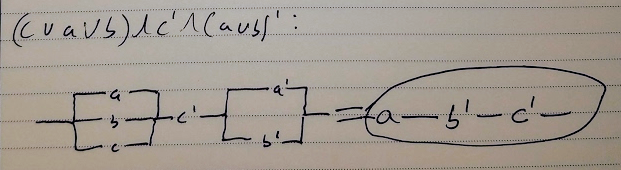
\includegraphics{Boolean4}}
\end{enumerate}
\end{document}